%%%%%%%%%%%%%%%%%%%%%%%%%%%%%%%%%%%%%%%%%%%%%%%%%%%%%%%%%%%%%%%%%%%%%%%%%%%%%%%%
\section{Benchmarking PDF moments}
\label{sec:benchmarking}
%%%%%%%%%%%%%%%%%%%%%%%%%%%%%%%%%%%%%%%%%%%%%%%%%%%%%%%%%%%%%%%%%%%%%%%%%%%%%%%%

In this section we provide a quantitative comparison between 
current lattice-QCD and global-fit results of the lowest
moments of unpolarized and polarized PDFs.
%
To this purpose, we identify benchmark quantities
and define the criteria to appraise the determinations
available in the literature.
%
For each benchmark quantity, we specify a prescription to 
select and combine lattice-QCD calculations and global-fit determinations.
%
We present our benchmark numbers from each side and compare them.

%%%%%%%%%%%%%%%%%%%%%%%%%%%%%%%%%%%%%%%%%%%%%%%%%%%%%%%%%%%%%%%%%%%%%%%%%%%%%%%%
\subsection{Benchmark criteria}
\label{subsec:BC}

We start by describing our benchmark criteria, which include the definition
of the benchmark quantities and the determination of their reference values,
based on a careful assessment of the lattice-QCD and global-fit results 
available in the literature.

\subsubsection{Benchmark quantities}
\label{subsubsec:BQ}

We identify our benchmark quantities with the following moments of unpolarized 
and polarized PDFs, or of PDF quark flavor combinations.
\begin{itemize}
  \item
$\langle x\rangle_{u^+-d^+}$, $\langle x \rangle_{u^+}$, $\langle x \rangle_{d^+}$, 
$\langle x \rangle_{s^+}$ and $\langle x \rangle_{g}$ in the unpolarized case; 
\item $g_A\equiv\langle 1 \rangle_{\Delta u^+ - \Delta d ^+}$, 
$\langle 1 \rangle_{\Delta u^+}$, $\langle 1 \rangle_{\Delta d^+}$,  
$\langle 1 \rangle_{\Delta s^+}$ and $\langle x \rangle_{\Delta u^- - \Delta d^-}$ 
  in the polarized case.
  \end{itemize}
%
We adopt the conventional notation described in Appendix~\ref{app:notation}.
%
We focus on the above quantities because current lattice 
calculations of higher moments and moments of other PDF 
combinations are not sufficiently controlled to allow for a meaningful 
comparison between lattice-QCD and global-fit results. 

\subsubsection{Appraising lattice-QCD calculations}
\label{subsubsec:BClQCD}

To accurately assess current lattice-QCD calculations
available in the literature, we follow a procedure inspired by the review of 
low-energy mesons undertaken by the Flavor Lattice Averaging Group 
(FLAG)~\cite{Aoki:2016frl}. 
%
For each lattice calculation, we characterize each source of 
uncertainty outlined in Sect.~\ref{Sec:IntroLQCD}. 
%
We use a rating system inspired by FLAG, awarding a blue star (\bstar) for 
sources of uncertainty that are well controlled or very conservatively 
estimated, a blue circle (\bcirc) for sources of uncertainty that have been 
controlled or estimated to some extent, and a red square (\rsquare) for 
uncertainties that have not met our criteria or for which no estimate is given.
%
Specifically, the rating system works as follows.

\begin{itemize}
\item {\bfseries Discretization effects and the continuum limit.}
We assume that the lattice actions are ${\cal O}(a)$-improved, {\it i.e.}, 
that the discretization errors vanish quadratically with the lattice spacing. 
%
For unimproved actions, an additional lattice spacing is required. 
%
These criteria must be satisfied in each case for at 
least one pion mass below 300~MeV.
%
\begin{itemize}
%
\item[\bstar] At least three lattice spacings with at least two lattice 
spacings below 0.1~fm and a range of lattice spacings that satisfies 
$[a_{\mathrm{max}}/a_{\mathrm{min}}]^2 \geq 2$.
%
\item[\bcirc] At least two lattice spacings with at least one point below 
0.1~fm and a range of lattice spacings that satisfy
$[a_{\mathrm{max}}/a_{\mathrm{min}}]^2 \geq 1.4$.
%
\end{itemize}
%
To receive a \bstar~or \bcirc~either a continuum extrapolation must be 
performed, or the results must demonstrate no significant discretization 
effects over the appropriate range of lattice spacings.

\item {\bfseries Unphysical pion masses.}
We define a physical pion mass ensemble to be one with $M_\pi=135\pm 10$~MeV
for the following criteria.
%
\begin{itemize}
\item[\bstar] One ensemble with a physical pion mass \emph{or} a chiral 
extrapolation with three or more pion masses, with at least two pion masses 
below 250~MeV and at least one below 200~MeV.
%
\item[\bcirc] A chiral extrapolation with three or more pion masses, two of 
which are below 300~MeV.
%
\end{itemize}

\item {\bfseries Finite-volume effects.}
%
For calculations that use a mixed-action approach, {\it i.e.},
with different lattice actions for the valence and sea quarks, 
we apply the following criteria to $M_\pi L$ for the valence quarks
($M_{\pi,\mathrm{min}}$ is the lightest pion mass employed in the calculation).
%
\begin{itemize}
%
\item[\bstar] Ensembles with $M_{\pi,\mathrm{min}}L\geq 4$, \emph{or} at least 
three volumes with spatial extent $L>2.5$~fm.
\item[\bcirc] Ensembles with $M_{\pi,\mathrm{min}}L \geq 3.4$, \emph{or} at least 
two volumes with spatial extent $L>2.5$~fm.
\end{itemize}

\item {\bfseries Excited-state contamination.}
%
\begin{itemize}
%
\item[\bstar] At least three source-sink separations or a variational method 
to optimize the operator derived from at least a $3\times 3$ correlator matrix, 
at every pion mass and lattice spacing.
% 
\item[\bcirc] Two source-sink separations at every pion mass and lattice 
spacing, or three or more source-sink separations at one pion mass below 
300~MeV.
%
For the variational method, an optimized operator derived from a $2\times 2$ 
correlator matrix at every pion mass and lattice spacing, or a $3\times 3$ 
correlator matrix for one pion mass below 300~MeV.
%
\end{itemize}

\item {\bfseries Renormalization.}
\begin{itemize}
%
\item[\bstar] Nonperturbative renormalization.
%
\item[\bcirc] Perturbative renormalization.
%
\end{itemize}
%
For $g_A$ we also award a \bstar~for calculations that use fermion actions 
for which $Z_A/Z_V=1$ or employ combinations of quantities for which the 
renormalization is unity by construction.

\item {\bfseries Lattice-spacing determination.}
For lattice-QCD calculations of nucleons, the lattice-spacing determination is 
generally sufficiently precise that it is a very small or negligible source
of systematic uncertainty. 
%
Therefore we do not include an assessment of the lattice-spacing
determination in our criteria.

\end{itemize}

Another important parameter in lattice-QCD calculations is the number of sea 
quark flavors, $N_f$. 
%
Following the approach used by FLAG, we prefer to avoid combining calculations 
with differing $N_f$; for more discussion of this issue, see the FLAG 
review~\cite{Aoki:2016frl}.

We now summarize the current status of lattice-QCD calculations of
our benchmark moments of unpolarized and polarized PDFs respectively.
%
Following FLAG, we consider only those results that are published in 
peer-reviewed journals or that have appeared as preprints. 
%
Where recent results are a clear update of previously published work, we do 
not include earlier results.
%
A bibliographical compilation of the results available in the literature 
is given for completeness in Appendix~\ref{sec:LQCDtables},
Tables~\ref{tab:latticebibfirst}-\ref{tab:latticebiblast}.
%
We characterize the results according to the criteria 
described above, and provide a prescription to combine those results that 
satisfy the criteria into a single benchmark value.

Our criteria and the corresponding ratings are chosen to provide not only as 
fair an assessment of the relative merits of various calculations as possible, 
but also a solid reference for future studies.
%
Where lattice-QCD results do not meet these standards, we hope that the lattice 
community will work towards improved calculations and greater precision.

\paragraph{Unpolarized parton distributions.}
We summarize the current status of lattice-QCD calculations of the benchmark 
moments of unpolarized PDFs listed in Sect.~\ref{subsubsec:BQ} in 
Table~\ref{tab:unpolLQCDstatus1}. 
%
We indicate: the computed moment in the first column; the collaboration who
performed the computation in the second column; the corresponding reference
in the third column; the number of sea quark flavors, $N_f$, in the fourth 
column.
%
We show whether the calculation has been published~(P) 
or has appeared as a preprint~(PreP) in the fifth column.
%
In the following five columns, we assess each source of systematic uncertainty
according to the criteria listed above. 
%
In the last column, we report the computed value at $\mu^2=4\mbox{ GeV}^2$
in the $\overline{{\rm MS}}$ scheme.
%
We refer the reader to the corresponding references for details on the 
meaning of the errors reported in parentheses.
%
We do not list results that have not been extrapolated to the physical pion 
mass, nor do we include quenched results in Table~\ref{tab:unpolLQCDstatus1}. 
%
For completeness, we report these results in  Appendix~\ref{sec:LQCDtables},
Table~\ref{tab:unpolLQCDstatus1B}.

%-------------------------------------------------------------------------------
\begin{table}[!t] 
\renewcommand{\arraystretch}{1.2} 
\centering 
\begin{threeparttable}
\begin{tabular}{llcllccccccl}
\toprule
Mom. & Collab. & Ref. & $N_f$ & Status & 
Disc &
QM &
FV &
Ren &
ES &
%
& Value\\
\midrule
$\langle x\rangle_{u^+-d^+}$ 
& LHPC\,14  
  & \cite{Green:2012ud} 
  & 2+1 
  & P  
  & \rsquare 
  & \bstar   
  & \bstar   
  & \bstar 
  & \bstar 
  & 
  & 0.140(21)\\
& ETMC 17  
  & \cite{Alexandrou:2017oeh} 
  & 2   
  & P
  & \rsquare 
  & \bstar   
  & \rsquare 
  & \bstar 
  & \bstar 
  & $^*$ 
  & 0.194(9)(11)\\
& RQCD 14  
  & \cite{Bali:2014gha} 
  & 2   
  & P  
  & \rsquare 
  & \rsquare 
  & \bcirc   
  & \bstar 
  & \bstar 
  & $^{**}$ 
  & 0.217(9)\\
\midrule
$\langle x\rangle_{u^+}$
&  ETMC 17  
  & \cite{Alexandrou:2017oeh} 
  & 2 
  & P
  & \rsquare 
  & \bstar   
  & \rsquare 
  & \bstar 
  & \bstar 
  & $^{*\triangleright}$ 
  & $0.453(57)(48)$\\
\midrule
$\langle x\rangle_{d^+}$
& ETMC 17  
  & \cite{Alexandrou:2017oeh} 
  & 2 
  & P
  & \rsquare 
  & \bstar   
  & \rsquare 
  & \bstar 
  & \bstar 
  & $^{*\triangleright}$ 
  & $0.259(57)(47)$\\
\midrule
$\langle x\rangle_{s^+}$
& ETMC 17  
  & \cite{Alexandrou:2017oeh} 
  & 2 
  & P
  & \rsquare  
  & \bstar   
  & \rsquare 
  & \bstar 
  & \bstar 
  & $^{*\triangleright}$ & $0.092(41)(0)$\\
\midrule
$\langle x\rangle_{g}$
& ETMC 17  
  & \cite{Alexandrou:2017oeh} 
  & 2 
  & P 
  & \rsquare 
  & \bstar   
  & \rsquare 
  & \bcirc 
  & \bstar 
  & $^*$ 
  & 0.267(22)(27)\\
\bottomrule
\end{tabular}
\begin{tablenotes}
\footnotesize
\item[$\ \,*$] Study employing a single physical pion mass ensemble.
\item[$**$] Study employing a single ensemble with $m_\pi=150$~MeV.
\item[$\ \,\triangleright$] Nonsinglet renormalization is applied.
%The mixing with $\langle x\rangle_{g}$ is computed.
\end{tablenotes}
\end{threeparttable}
\caption{\small Status of current lattice-QCD calculations of the benchmark 
first moments of unpolarized PDFs listed in Sect.~\ref{subsubsec:BQ}.
%
A detailed description of each entry, including the symbols used to 
characterize the various sources of systematics, is provided in the text.
%
Values are shown at $\mu^2=4\mbox{ GeV}^2$.
%
We refer the reader to the corresponding references for details on the 
errors reported in parentheses.
%
To denote the various sources of systematic uncertainty, 
we use the abbreviations Disc (discretization),
QM (quark mass), FV (finite volume),
Ren (renormalization) and ES (excited states).
%
}
\label{tab:unpolLQCDstatus1}
\end{table}
%-------------------------------------------------------------------------------

As is apparent from Table~\ref{tab:unpolLQCDstatus1}, there are no lattice 
calculations of the considered first moments for which all systematics 
have been fully explored and controlled.  
%
In the case of $\langle x\rangle_{u^+-d^+}$ three different results are available 
in the literature.
%
We present the lattice-QCD benchmark value for this quantity 
as a best-estimate band.
% 
This band extends from the mean of the smallest result minus its error 
to the mean of the largest result plus its error, and includes all results 
listed in Table~\ref{tab:unpolLQCDstatus1} with two or more sea 
quark flavors.
%
Current studies are not sufficiently precise to distinguish between 
results with different numbers of sea quark flavors.
%
In the case of $\langle x \rangle_{u^+}$, $\langle x \rangle_{d^+}$, 
$\langle x \rangle_{s^+}$ and $\langle x \rangle_g$, there is only one
lattice result available in the literature:
for these quantities, our lattice-QCD benchmark value is the single result; 
however, it should be noted that these results may underestimate some sources 
of uncertainty. 

The lattice-QCD benchmark numbers for $\langle x\rangle_{u^+-d^+}$,
$\langle x \rangle_{u^+}$, $\langle x \rangle_{d^+}$, 
$\langle x \rangle_{s^+}$ and $\langle x \rangle_g$ will be further
commented below, where they will be collected together with their 
global-fit counterparts in Table~\ref{tab:BMunp}.

Finally, we summarize the current status of lattice-QCD calculations of the 
second moment of the unpolarized valence-quark PDFs, 
$\langle x^2 \rangle_{u^-}$, $\langle x^2 \rangle_{d^-}$ and 
$\langle x^2\rangle_{u^--d^-}$ in Appendix~\ref{sec:LQCDtables},
Table~\ref{tab:unpolLQCDstatus2B}.
% 
The study of these moments is not sufficiently mature to provide benchmark 
values and we only list the results for completeness.

\paragraph{Polarized parton distributions.}
The zeroth moment of the isotriplet polarized PDF combination is related to the 
axial charge of the nucleon, $g_A\equiv \langle 1\rangle_{\Delta u^+-\Delta d^+}$.
%
This quantity is of central importance to nucleon physics and has long been 
considered an important benchmark for lattice calculations. 
%
Historically, lattice-QCD calculations of the axial charge have underestimated 
the experimental value $g_A^{\mathrm{exp}} = 1.2723(23)$~\cite{Olive:2016xmw}
(see also Eq.~\eqref{eq:a3}), 
which is most precisely determined from neutron weak decays. 
%
Thus, the axial charge has been the single most-studied moment in lattice QCD.
%
We summarize the current status of these calculations in 
Table~\ref{tab:gAstatus} using the same format as in 
Table~\ref{tab:unpolLQCDstatus1}.
%
All results are quoted at $\mu^2=4\mbox{ GeV}^2$.

%-------------------------------------------------------------------------------
\begin{table}[!t]
\renewcommand{\arraystretch}{1.2} 
\centering
\begin{threeparttable}
\begin{tabular}{llcllccccccl}
\toprule
Mom. & Collab. & Ref. & $N_f$ & Status &  
Disc &
QM &
FV &
Ren &
ES &
%
& Value \\
\midrule
$g_A$
& CalLat\,17 
  & \cite{Berkowitz:2017gql} 
  & 2+1+1 
  & PreP 
  & \rsquare 
  & \bstar  
  & \rsquare 
  & \bstar 
  & \bstar 
  & %$^\diamond$ 
  & 1.278(21)(26) \\
& PNDME\,16  
  & \cite{Bhattacharya:2016zcn} 
  & 2+1+1 
  & P    
  & \bcirc   
  & \bstar  
  & \bcirc   
  & \bstar 
  & \bstar 
  & 
  & 1.195(33)(20)\\
& LHPC\,14    
  & \cite{Green:2012ud} 
  & 2+1 
  & P 
  & \rsquare 
  & \bstar 
  & \bstar 
  & \bstar  
  & \bstar & & 0.97(8)\\
& Mainz\,17   
  & \cite{Capitani:2017qpc} 
  & 2 
  & PreP 
  & \bstar 
  & \bcirc 
  & \bstar 
  & \bstar  
  & \bstar 
  & 
  & $1.278(68)({}^{+0}_{-0.087})$\\
& ETMC\,17    
  & \cite{Alexandrou:2017hac} 
  & 2 
  & P
  & \rsquare  
  & \bstar 
  & \rsquare  
  & \bstar  
  & \bstar 
  & $^*$ 
  & 1.212(33)(22)\\
& RQCD\,15    
  & \cite{Bali:2014nma} 
  & 2 
  & P 
  & \bcirc 
  & \bcirc  
  & \bcirc  
  & \bstar   
  & \bcirc 
  & $^\ddag$
  & 1.280(44)(46) \\
  & QCDSF\,14   
  & \cite{Horsley:2013ayv} 
  & 2 
  & P 
  & \bcirc 
  & \bcirc  
  & \bcirc  
  & \bstar  
  & \rsquare 
  & $^\ddag$
  & 1.29(5)(3) \\
\bottomrule
\end{tabular}
\begin{tablenotes}
\footnotesize
\item[$*$] Study employing a single physical pion mass ensemble.
\item[$^\ddag$] $g_A$ is determined via the ratio $g_A/f_\pi$, employing the 
physical value for $f_\pi$.
%\item[$\diamond$] Approach inspired by the Feynman-Hellmann method.
\end{tablenotes}
\end{threeparttable}
\caption{\small Same as Table~\ref{tab:unpolLQCDstatus1}, but for the axial 
coupling, $g_A\equiv \langle 1\rangle_{\Delta u^+-\Delta d^+}$. 
%
Studies with three or more red squares are omitted from this table.
%
Values are shown at $\mu^2=4\mbox{ GeV}^2$.
%
}
\label{tab:gAstatus}
\end{table}
%-------------------------------------------------------------------------------

As is apparent from Table~\ref{tab:gAstatus}, we consider 
only three calculations of $g_A$ to have all systematics
sufficiently controlled to obtain a blue circle or star.
%
One of them~\cite{Bhattacharya:2016zcn} is for $N_f=2+1+1$, while two of 
them~\cite{Capitani:2017qpc,Bali:2014nma} are for $N_f=2$.
%
In the former case, our benchmark value corresponds to the single calculation;
in the latter case, our benchmark value corresponds to a weighted average 
of \cite{Capitani:2017qpc} and \cite{Bali:2014nma}, assuming correlations
between the results, and applying the procedure of \cite{Schmelling:1994pz}.
%
In summary, our benchmark values are
\begin{equation}\label{eq:gAcriteria}
g_A^{N_f=2+1+1} = 1.195(33)(20)
\,,\qquad \mathrm{and}\qquad 
g_A^{N_f=2} = 1.279(50)\,.
\end{equation}

We observe that the result of~\cite{Berkowitz:2017gql}, although it does
not fulfill all our requirements on systematic uncertainties, uses the same 
gauge configurations as those of \cite{Bhattacharya:2016zcn}.
%
Therefore, we also carry out a simultaneous fit to the two results for
completeness.
%
We use a fit function of the form
\begin{eqnarray}
g_A^{\mathrm{fit}}
&=&
c_0 +
f(a) +
c_3M_\pi^2 +
c_4M_\pi^2 \exp(-M_\pi L) +
c_5M_\pi^2 \log\left(\frac{M_\pi^2}{\Lambda_{\chi \mathrm{PT}}^2}\right)\,,
\\
f(a) &=&
\begin{cases}
  c_1a   & \qquad \text{Ref.~\cite{Bhattacharya:2016zcn}} \\
  c_2a^2 & \qquad \text{Ref.~\cite{Berkowitz:2017gql}}\\
\end{cases}
\qquad .
\end{eqnarray}
%
The coefficient $c_1$ captures ${\cal O}(a)$ effects present in the
valence-quark action of~\cite{Bhattacharya:2016zcn}, while~\cite{Berkowitz:2017gql} 
has discretization effects starting at ${\cal O}(a^2)$. 
%
The term proportional to $c_4$ captures the leading finite-volume effects, and 
$c_3$ and $c_5$ represent chiral-extrapolation terms. 
%
Modifications to this fit form, including setting $c_5=0$, have a negligible 
effect on the fit results within extrapolation uncertainties, and the final 
result is in very good agreement with a weighted average of the two 
calculations, assuming 100\% correlations, which is 
$g_A^{N_f=2+1+1,\mathrm{avg}} = 1.243(36)$. 
%
Based on this fit, we find the best-estimate band of
\begin{equation}\label{eq:gAfit}
g_A^{N_f=2+1+1,\mathrm{fit}} = \numrange{1.22}{1.28}\,.
\end{equation}

We plot all lattice results for the axial coupling, listed in 
Table~\ref{tab:gAstatus}, in Fig.~\ref{fig:gaLQCDstatus}. 
%
We show the world-average experimental value as a vertical black line. 
%
The light gray bands for $N_f=2+1+1$ and $N_f=2$ represent the benchmark 
results of Eq.~\eqref{eq:gAcriteria}, and the dashed gray band for
$N_f=2+1+1$ is the combined fit band given in Eq.~\eqref{eq:gAfit}. 

%-------------------------------------------------------------------------------
\begin{figure}[!t]
\centering
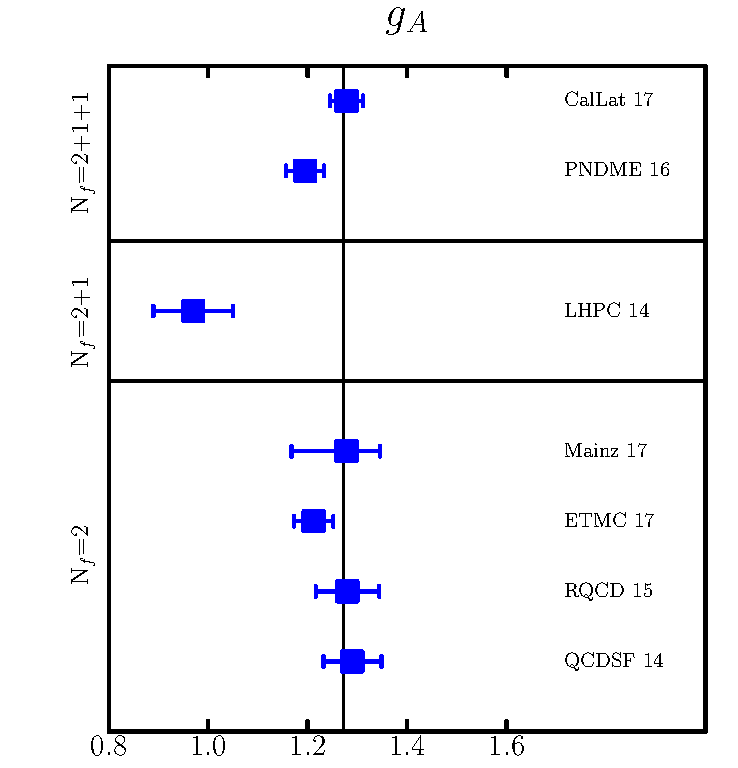
\includegraphics[scale=0.7]{plots/ga_summary.pdf}\\
\caption{\small Summary of the current status of lattice-QCD calculations of 
the axial charge, $g_A\equiv \langle 1\rangle_{\Delta u^+-\Delta d^+}$.
%
The vertical black line represents the current experimental world average 
$g_A^{\mathrm{exp}} = 1.2723(23)$~\cite{Olive:2016xmw}. 
%
The light gray bands for $N_f=2+1+1$ and $N_f=2$ represent the benchmark 
results of Eq.~\eqref{eq:gAcriteria}, and the dashed gray band for
$N_f=2+1+1$ is the fit band of Eq.~\eqref{eq:gAfit}.}    
\label{fig:gaLQCDstatus}
\end{figure}
%-------------------------------------------------------------------------------

In addition to the axial charge, we summarize the zeroth moments of the 
individual light-quark total polarized distributions in 
Table~\ref{tab:polLQCDstatus0}. 
%
We summarize the status of lattice-QCD calculations of the
first moments of the polarized PDF combination 
$\langle x \rangle_{\Delta u^- - \Delta d^-}$ in Table~\ref{tab:polLQCDstatus1}. 
%
We use the same format as in Table~\ref{tab:unpolLQCDstatus1}.
%
All values are at $\mu^2=4\mbox{ GeV}^2$.
%
Available results that have not been extrapolated to the physical pion mass
or quenched results are not reported here, but in Appendix~\ref{sec:LQCDtables},
Tables~\ref{tab:polLQCDstatus1B}-\ref{tab:polLQCDstatus2B}, for completeness.

In the case of $\langle 1 \rangle_{\Delta u^+}$ and $\langle 1 \rangle_{\Delta d^+}$,
there is only one result available in the literature for each quantity.
%
Therefore, although the corresponding systematic uncertainties are not 
completely under control and possibly underestimated, we take the individual 
results as our benchmark values.
%
In the case of $\langle 1 \rangle_{\Delta s^+}$ and 
$\langle x \rangle_{\Delta u^- - \Delta d^-}$, however, several results are available
in the literature, although without a full characterization of
their systematic uncertainties.
%
We present our lattice-QCD benchmark value for these quantities as
a best-estimate band extending from the mean minus the error of the 
smallest result to the mean plus the error of the largest. 
%
We include all results with two or more flavors of sea quarks listed in 
Tables~\ref{tab:polLQCDstatus0} and \ref{tab:polLQCDstatus1}, respectively.

The lattice-QCD benchmark numbers for $g_A$,
$\langle 1 \rangle_{\Delta u^+}$, $\langle 1 \rangle_{\Delta d^+}$,
$\langle 1 \rangle_{\Delta s^+}$ and $\langle x \rangle_{\Delta u^- - \Delta d^-}$
will be further commented below, where they will be collected together 
with their global-fit counterparts in Table~\ref{tab:BMpol}.

%-------------------------------------------------------------------------------
\begin{table}[!t]
\renewcommand{\arraystretch}{1.2} 
\centering
\begin{threeparttable}
\begin{tabular}{llcllccccccl}
\toprule
Mom. & Collab. & Ref. & $N_f$ & Status &
Disc &
QM &
FV &
Ren &
ES &
%
& Value \\
\midrule
$\langle 1\rangle_{\Delta u^+}$
& ETMC\,17 
  & \cite{Alexandrou:2017oeh} 
  & 2 
  & P
  & \rsquare 
  & \bstar 
  & \rsquare 
  & \bstar 
  & \bstar 
  & $^*$ 
  & $0.830(26)(4)$\\
\midrule
$\langle 1\rangle_{\Delta d^+}$
& ETMC\,17  
  & \cite{Alexandrou:2017oeh} 
  & 2 
  & P
  & \rsquare 
  & \bstar 
  & \rsquare  
  & \bstar 
  & \bstar 
  & $^*$ 
  & $-0.386(16)(6)$\\
\midrule
$\langle 1\rangle_{\Delta s^+}$
& $\chi$QCD\,17 
  & \cite{Gong:2015iir} 
  & 2+1 
  & P 
  & \rsquare  
  & \bcirc 
  & \bcirc  
  & \bstar 
  & \bstar
  & $^{\dagger,\triangleleft}$ 
  & -0.0403(44)(78)\\
& Engelhardt\,12 
  & \cite{Engelhardt:2012gd} 
  & 2+1 
  & P 
  & \rsquare  
  & \rsquare 
  & \bcirc  
  & \bstar  
  & \bstar  
  & $^\triangleleft$ 
  & -0.031(17)\\
& ETMC\,17 
  & \cite{Alexandrou:2017oeh} 
  & 2 
  & P
  & \rsquare  
  & \bstar 
  & \rsquare  
  & \bstar  
  & \bstar 
  & $^*$ 
  & -0.042(10)(2)\\
\bottomrule
\end{tabular}
\begin{tablenotes}
\footnotesize
\item[$*$] Study employing a single physical pion mass ensemble.
\item[$\dagger$] Partially quenched simulation with $m_\pi=330$~MeV. 
Criteria applied to the valence quarks. 
\item[$\triangleleft$] Some parts of the renormalization are estimated, 
see references for details.
\end{tablenotes}
\end{threeparttable}
\caption{\small Same as Table~\ref{tab:unpolLQCDstatus1}, but for the 
zeroth moments of the polarized total quark distributions.
%
Values are shown at $\mu^2=4\mbox{ GeV}^2$.
}
\label{tab:polLQCDstatus0}
\end{table}
%-------------------------------------------------------------------------------

%-------------------------------------------------------------------------------
\begin{table}[!t] 
\renewcommand{\arraystretch}{1.2}
\centering
\begin{threeparttable}
\begin{tabular}{llcllccccccl}
\toprule
Mom. & Collab. & Ref. & $N_f$ & Status &
Disc &
QM &
FV &
Ren &
ES &
& Value \\
\midrule
$\langle x\rangle_{\Delta u^--\Delta d^-}$
& RBC/ 
  & \multirow{2}{*}{\cite{Aoki:2010xg}} 
  & \multirow{2}{*}{2+1} 
  & \multirow{2}{*}{P} 
  & \multirow{2}{*}{\rsquare}  
  & \multirow{2}{*}{\rsquare} 
  & \multirow{2}{*}{\bstar}  
  & \multirow{2}{*}{\bstar}  
  & \multirow{2}{*}{\rsquare} 
  &  
  & 0.256(23)/\\
& UKQCD\,10 
  &  
  &  
  &  
  &   
  &  
  &   
  &   
  &  
  &  
  & 0.205(59)\\
& LHPC\,10 
  & \cite{Bratt:2010jn} 
  & 2+1 
  & P 
  & \rsquare  
  & \rsquare 
  & \bcirc  
  & \bcirc  
  & \rsquare 
  &  
  & 0.1972(55)\\
& ETMC\,15 
  & \cite{Abdel-Rehim:2015owa} 
  & 2 
  & P 
  & \rsquare  
  & \bstar 
  & \rsquare  
  & \bstar  
  & \bstar 
  & $^*$ 
  & 0.229(33)\\
\bottomrule
\end{tabular}
\begin{tablenotes}
\footnotesize
\item[$*$] Study employing a single physical pion mass ensemble.
\end{tablenotes}
\end{threeparttable}
\caption{\small Same as Table~\ref{tab:unpolLQCDstatus1}, but for the 
first moment of the polarized valence-quark distribution.
%
Values are shown at $\mu^2=4\mbox{ GeV}^2$.
}
\label{tab:polLQCDstatus1}
\end{table}
%-------------------------------------------------------------------------------

\subsubsection{Appraising global-fit results}
\label{subsubsec:GPDFfits}

The current status of global PDF fit determinations and their 
uncertainties has been carefully assessed in dedicated reviews
recently~\cite{Forte:2013wc,Jimenez-Delgado:2013sma}, and further 
summarized in Sect.~\ref{sec:unpPDFs}. 
%
It is now recognized that PDF uncertainties receive various contributions: 
the measurement uncertainty propagated from the data, uncertainties associated 
with incompatible data sets, procedural uncertainties such as those related to 
the choice of the PDF parametrization, 
and the handling of systematic errors, among others.
%
As outlined in Sect.~\ref{sec:unpPDFs}, in principle all of these uncertainties 
can be accounted for with suitable methods, both in the Hessian and the 
MC frameworks.
%
In practice, there is a significant spread in the sophistication 
of these methods between unpolarized and polarized PDF fits.

In Sect.~\ref{sec:unpPDFs}, we also emphasized that there are additional 
theoretical uncertainties on PDFs associated with uncertainty in
the input values of the physical parameters used in the fit (such as the 
reference value of the strong coupling) and with missing higher-order
uncertainties (given that fits are usually performed with fixed-order
perturbation theory).
%
The size of the former can be accounted for by studying the stability of the 
results upon variation of the input parameters; the size of the latter is
currently unknown, although it is supposed to be sub-dominant.
%
Therefore, theoretical uncertainties will not be considered in the following.

As far as full moments of PDFs are concerned, global-fit results involve
some degree of extrapolation to the region not covered by experimental data, 
that is not necessarily well accounted for in the PDF error estimates.
%
Extrapolation is particularly delicate to small $x$ values in the case of 
polarized PDFs: opposite to unpolarized PDFs, the kinematic coverage is 
fairly limited (see Sect.~\ref{sec:polPDFs} and in particular 
Fig.~\ref{fig:kinEIC}) and there is no analog of the momentum sum rule,
Eq.~\eqref{eq:mom}, to further constrain the PDFs.
%
Extrapolation uncertainties are difficult to quantify, unless
one naively extrapolates uncertainty bands from the measured region.

We now summarize the results for our benchmark moments listed in 
Sect.~\ref{subsubsec:BQ}, based on current global-fit determinations of
unpolarized and polarized PDFs.
%
We specify how the
available results are combined into a single benchmark value.

\paragraph{Unpolarized parton distributions.}

We summarize the current status of global-fit results of the benchmark
moments of unpolarized PDFs listed in Sect.~\ref{subsubsec:BQ} 
in Table~\ref{tab:unpPDFmoms}.
%
In the first column we indicate the computed moment, and in the subsequent 
six columns the moment's value, obtained from the most recent available PDF 
determinations: NNPDF3.1~\cite{Ball:2017nwa},
CT14~\cite{Dulat:2015mca}, MMHT2014~\cite{Harland-Lang:2014zoa},
ABMP16~\cite{Alekhin:2017kpj} (with $N_f=4$ flavors), 
CJ15~\cite{Accardi:2016qay} and 
HERAPDF2.0~\cite{Abramowicz:2015mha} respectively.
%
The most relevant features of these PDF sets have been presented in 
Sect.~\ref{sec:unpPDFs}.
%
All values in Table~\ref{tab:unpPDFmoms} are displayed
at $\mu^2=4\mbox{ GeV}^2$. 
%
They have been obtained from the default PDF sets at the highest available 
perturbative order, which is NNLO for all of them except CJ15
for which it is NLO.
%
The uncertainties for the CT14 PDF set has been rescaled by a factor $1/1.65$ 
to convert from  90\%-CL bands to  68\%-CL bands.
%
Note that tolerance of $\Delta \chi^2=1$ at 68\% CL is used in the CJ15 PDF 
set; hence, the smaller uncertainties of this set compared to all the other 
PDF sets.
%
Also, the CJ15 set does  not fit $\langle x \rangle_{s^+}$, therefore the 
corresponding number is not displayed in Table~\ref{tab:unpPDFmoms}. 
%
In the case of the HERAPDF2.0 set, the error band is the sum in quadrature 
of the statistical, model and parametrization uncertainties.
%
Taking the results of Table~\ref{tab:unpPDFmoms} at face value,
there are clear discrepancies arising from a variety of 
factors~\cite{Butterworth:2015oua,Accardi:2016ndt};
we examine some of these in the following. 

%-------------------------------------------------------------------------------
\begin{table}[!t]
\centering
\renewcommand{\arraystretch}{1.2}
\begin{tabular}{lcccccc}
\toprule
Mom. 
& NNPDF3.1 & CT14 & MMHT2014 & ABMP2016 & CJ15 & HERAPDF2.0 \\
\midrule
$\langle x \rangle_{u^+-d^+}$ 
& 0.152(3) & 0.158(4) & 0.151(4) & 0.167(4) & 0.152(2) & 0.188(3)\ \,\\
$\langle x \rangle_{u^+}$    
& 0.348(4) & 0.348(3) & 0.348(5) & 0.353(3) & 0.348(1) & 0.372(4)\ \,\\
$\langle x \rangle_{d^+}$    
& 0.196(3) & 0.190(3) & 0.197(5) & 0.186(3) & 0.196(1) & 0.185(7)\ \,\\
$\langle x \rangle_{s^+}$    
& 0.039(3) & 0.035(5) & 0.035(9) & 0.041(2) & ---   & 0.035(11)\\
$\langle x \rangle_{g}$     
& 0.410(4) & 0.416(5) & 0.411(9) & 0.412(4) & 0.416(1) & 0.401(10)\\
\bottomrule
\end{tabular}
\caption{\small Status of current global PDF fit determinations of the 
benchmark moments of unpolarized PDFs listed in Sect.~\ref{subsubsec:BQ}.
All values are shown at $\mu^2=4\mbox{ GeV}^2$.
%
See text for details about the calculation of PDF uncertainties in each case.
}
\label{tab:unpPDFmoms}
\end{table}
%-------------------------------------------------------------------------------

In order to provide a benchmark value for the first moments of unpolarized PDFs
listed in Table~\ref{tab:unpPDFmoms}, we follow the latest PDF4LHC 2015 
recommendations~\cite{Butterworth:2015oua}.
%
Even though the recommendations were primarily formulated for the usage of PDFs
in LHC-related physics, and alternative recommendations have been 
suggested~\cite{Accardi:2016ndt}, we find it useful to apply them here as well.
%
The reason is twofold.
%
First, this benchmark exercise aims at accuracy and precision,  
two of the guiding principles underlying the recommendations.
%
Second, they led to the release of a specific PDF set
that can be easily used to compute all the needed benchmark values.

While we refer the reader to \cite{Butterworth:2015oua} for details,
here we only mention that the PDF4LHC15 PDF set was constructed by means of
a statistical combination~\cite{Carrazza:2015hva,Gao:2013bia,Watt:2012tq,
Carrazza:2015aoa} (an unweighted average) of the 
NNPDF3.0~\cite{Ball:2014uwa}, CT14 and MMHT2014 PDF sets.\footnote{The 
NNPDF3.1 PDF set was not available when the recommendations were formulated.}
%
The three PDF sets were selected among all the publicly available PDF sets
based on four criteria~\cite{Butterworth:2015oua}.
%
\begin{itemize}
%
\item A global data set from a wide variety of observables and processes
should be included in the fit analysis.
%
\item Theoretical hard cross sections should be evaluated up to NNLO in a
general-mass variable-flavor number scheme with up to $N_f^\text{max}=5$ 
active quark flavors.
%
\item The central value of the strong coupling at the $Z$-boson mass,
$\alpha_s(M_Z^2)$ should be fixed at an agreed common value, consistent 
with the PDG world-average~\cite{Olive:2016xmw} ($\alpha_s(M_Z)=0.118$).
%
\item All known experimental and procedural sources of uncertainty should be 
properly accounted for.
%
\end{itemize}
%
The ABMP2016 set (as well as its previous versions) does not meet the second 
and third criteria; the CJ15 set does not meet the first, second and fourth
criteria, while the HERAPDF2.0 set does not meet the first criterion.
%
Hence, these sets were not included in the PDF4LHC2015 PDF set, although the 
possibility of including them in future versions of the recommendation 
remains open.

In order not to loose important information contained in the PDF sets excluded 
from the PDF4LHC recommendations, we also provide alternative benchmark numbers.
%
Specifically, we combined all the numbers quoted in Table~\ref{tab:unpPDFmoms}
so that the mean value is an unweighted average of the mean 
values and the error is half of the difference between the smallest and the 
largest result.
%
The rationale for this choice is that PDF sets entering the PDF4LHC 
recommendations are not benchmarked in the $x\gtrsim 0.1$ region, which can be 
relevant for the moment analysis.
%
The combination of all results in Table~\ref{tab:unpPDFmoms}, although 
sometimes less precise than the PDF4LHC combination, maximizes the amount of 
experimental information included in the benchmark numbers.
%
Specifically, it includes the information taken into account 
at large $x$ and small $Q^2$ in the CJ15 and ABMP16 PDF sets, 
which is otherwise excluded from the PDF4LHC set.

The global-fit benchmark numbers for $\langle x\rangle_{u^+-d^+}$,
$\langle x \rangle_{u^+}$, $\langle x \rangle_{d^+}$, 
$\langle x \rangle_{s^+}$ and $\langle x \rangle_g$ will be further
commented below, where they will be collected together with their 
lattice-QCD counterparts in Table~\ref{tab:BMunp}.

\paragraph{Polarized parton distributions.}
%
We summarize the current status of global-fit results of the benchmark
moments of polarized PDFs listed in Sect.~\ref{subsubsec:BQ} in 
Table~\ref{tab:polPDFmoms}.
%
In the first column, we indicate the computed moment, and in the subsequent 
three columns, its value as obtained from the most recent available PDF 
determinations: NNPDFpol1.1~\cite{Nocera:2014gqa}, 
DSSV08~\cite{deFlorian:2009vb}~\footnote{The DSSV08 analysis has been updated
by the DSSV14 analysis~\cite{deFlorian:2014yva} essentially 
only in the determination of the gluon PDF. 
The moments in Table~\ref{tab:polPDFmoms} therefore hardly differ
in the two analyses.}, JAM15~\cite{Sato:2016tuz} and 
JAM17~\cite{Ethier:2017zbq}.
%
The most relevant features of these PDF sets have been presented in
Sect.~\ref{sec:polPDFs}.
%
All values in Table~\ref{tab:unpPDFmoms} are displayed
at $\mu^2=4\mbox{ GeV}^2$ at NLO.
%
The uncertainties correspond to 68\%-CL bands with tolerance of 
$\Delta \chi^2=1$ for the DSSV08 PDF set.
%
In the case of the JAM15 set, we do not provide a value for 
$\langle x \rangle _{\Delta u^--\Delta d^-}$:
the fit is based on inclusive DIS data only, which are not sensitive to 
the valence distribution $\Delta u^- - \Delta d^-$.
%
We emphasize that, because of extrapolation uncertainties difficult to quantify,
the error estimates in Table~\ref{tab:polPDFmoms} should be interpreted
as a lower bound, especially for the DSSV08 and JAM sets based on 
conventional parametrizations.
%
In these cases, uncertainty bands are naively extrapolated from the measured 
kinematic region, therefore they are likely to underestimate the contribution 
coming from the small-$x$ region.

%-------------------------------------------------------------------------------
\begin{table}[!t]
\centering
\renewcommand{\arraystretch}{1.2}
\begin{tabular}{lcccc}
\toprule
Mom. 
& NNPDFpol1.1 & DSSV08 & JAM15 & JAM17 \\
\midrule
$\langle 1 \rangle_{\Delta u^+-\Delta d^+}$ &
\ 1.250(16) & \ 1.260(18) & 1.314(6)\,  & \ 1.240(41)\\
$\langle 1 \rangle_{\Delta u^+}$ &
\ 0.794(46) & \ 0.814(12) & \ 0.831(21) & \ 0.812(22)\\
$\langle 1 \rangle_{\Delta d^+}$ &  
-0.453(52)  &  -0.456(11) &  -0.476(22) &  -0.428(31)\\
$\langle 1 \rangle_{\Delta s^+}$ &  
-0.120(81)  &  -0.112(23) &  -0.109(20) &  -0.038(96)\\
$\langle x \rangle_{\Delta u^- - \Delta d^-}$ &     
\ 0.195(14) &  0.203(9)\, &  ---        & \ 0.241(26)\\
\bottomrule
\end{tabular}
\caption{\small Status of current global-fit determinations of the 
benchmark moments of polarized PDFs listed in Sect.~\ref{subsubsec:BQ}.
All values are shown at $\mu^2=4\mbox{ GeV}^2$.}
\label{tab:polPDFmoms}
\end{table}
%-------------------------------------------------------------------------------

As outlined in Sect.~\ref{sec:polPDFs}, polarized PDFs cannot be determined in 
a global QCD analysis with the same accuracy as their unpolarized counterparts.
%
Also, because polarized PDFs do not enter precision physics studies at the LHC, 
the selection and combination of different PDF sets has received much less
attention.
%
No recommendations analogous to those from the PDF4LHC working group
exist for polarized PDFs.

To provide a benchmark value for the relevant moments of 
polarized PDFs listed in Table~\ref{tab:polPDFmoms}, we apply an unweighted 
average of the NNPDFpol1.1, DSSV08 and JAM15 PDF sets.
%
The rationale for this choice is twofold.
%
On the one hand, we maximize the amount of experimental information 
that can determine the central value of our benchmark moments.
%
As explained in Sect.~\ref{sec:polPDFs}, the NNPDFpol1.1 and the DSSV08 PDF 
sets are based on a very similar set of inclusive DIS data, while the JAM15 
PDF set is based on a much wider inclusive DIS data set.
%
This wider set can help constrain the moments of the total quark 
distributions.
%
The NNPDFpol1.1 and the DSSV08 PDF sets are based respectively on $pp$ and 
SIDIS data to disentangle the quark and antiquark distributions.
%
This can help constrain the moments of the valence distributions.
%
On the other hand, we balance the rather different uncertainties among the 
three PDF sets, specifically the larger NNPDFpol1.1 estimate
against the smaller DSSV08 and JAM15 values.
%
This way, we avoid a possible underestimation of the procedural uncertainties 
induced for example by the choice of a simple PDF parametrization 
in the DSSV08 and JAM15 fits, or by the extrapolation to the small-$x$ region.
%
Because the JAM17 set is unique in fitting simultaneously polarized PDFs and 
FFs, we do not include it in our benchmark average, but quote it as a useful 
comparison.

The global-fit benchmark numbers for $g_A$,
$\langle 1 \rangle_{\Delta u^+}$, $\langle 1 \rangle_{\Delta d^+}$,
$\langle 1 \rangle_{\Delta s^+}$ and $\langle x \rangle_{\Delta u^- - \Delta d^-}$
will be further commented below, where they will be collected
with their lattice-QCD counterparts in Table~\ref{tab:BMpol}.

%%%%%%%%%%%%%%%%%%%%%%%%%%%%%%%%%%%%%%%%%%%%%%%%%%%%%%%%%%%%%%%%%%%%%%%%%%%%%%%%
\subsection{Comparing lattice-QCD and global-fit benchmark moments}
\label{subsec:BN}

We can now compare the lattice-QCD and global PDF fit results presented in 
Sects.~\ref{subsubsec:BClQCD}-\ref{subsubsec:GPDFfits} for the unpolarized
and polarized PDF moments respectively.

\paragraph{Unpolarized parton distributions.}
%
The benchmark values of the first moments of the unpolarized PDFs, obtained
as described in Sects.~\ref{subsubsec:BClQCD}-\ref{subsubsec:GPDFfits}, 
are summarized in Table~\ref{tab:BMunp}.
%
Both the PDF4LHC and the unweighted average (uw avg) are displayed in the case 
of global fits.
%
The results from a single lattice calculation, which might underestimate some 
sources of uncertainty, are denoted with a superscript~$\dagger$.
%
All values shown here are at $\mu^2=4\mbox{ GeV}^2$.
%
For ease of comparison, these benchmark results are also graphically
compared in Fig.~\ref{fig:Bmomsunp}, both in terms of absolute values 
(left panel) and of uncorrelated ratios to the lattice central values 
(right panel).

%-------------------------------------------------------------------------------
\begin{table}[!t]
\centering
\renewcommand{\arraystretch}{1.2}
\begin{tabular}{lccc}
\toprule
Moment & Lattice QCD & Global Fit (PDF4LHC) & Global fit (uw avg)\\
\midrule
$\langle x \rangle_{u^+ -d^+}$ 
& \numrange{0.119}{0.226} 
& 0.155(5)
& \, 0.161(18)\\
$\langle x \rangle_{u^+}$     
& 0.453(75)$^\dagger$ 
& 0.347(5)
& \, 0.352(12)\\
$\langle x \rangle_{d^+}$     
& 0.259(74)$^\dagger$ 
& 0.193(6)
& 0.192(6)\\
$\langle x \rangle_{s^+}$     
& 0.092(41)$^\dagger$ 
& 0.036(6)
& 0.037(3)\\
$\langle x\rangle_{g}$       
& 0.267(35)$^\dagger$ 
& 0.414(9)
& 0.411(8)\\
\bottomrule
\end{tabular}
\caption{\small Benchmark values for lattice-QCD calculations and global-fit 
determinations of the benchmark moments of unpolarized PDFs.
%
All values are shown at $\mu^2=4\mbox{ GeV}^2$.
%
Results with a superscript~$\dagger$ are from a single lattice 
calculation; they may underestimate some sources of uncertainty.}
\label{tab:BMunp}
\end{table}
%-------------------------------------------------------------------------------

%-------------------------------------------------------------------------------
\begin{figure}[!t]
\centering
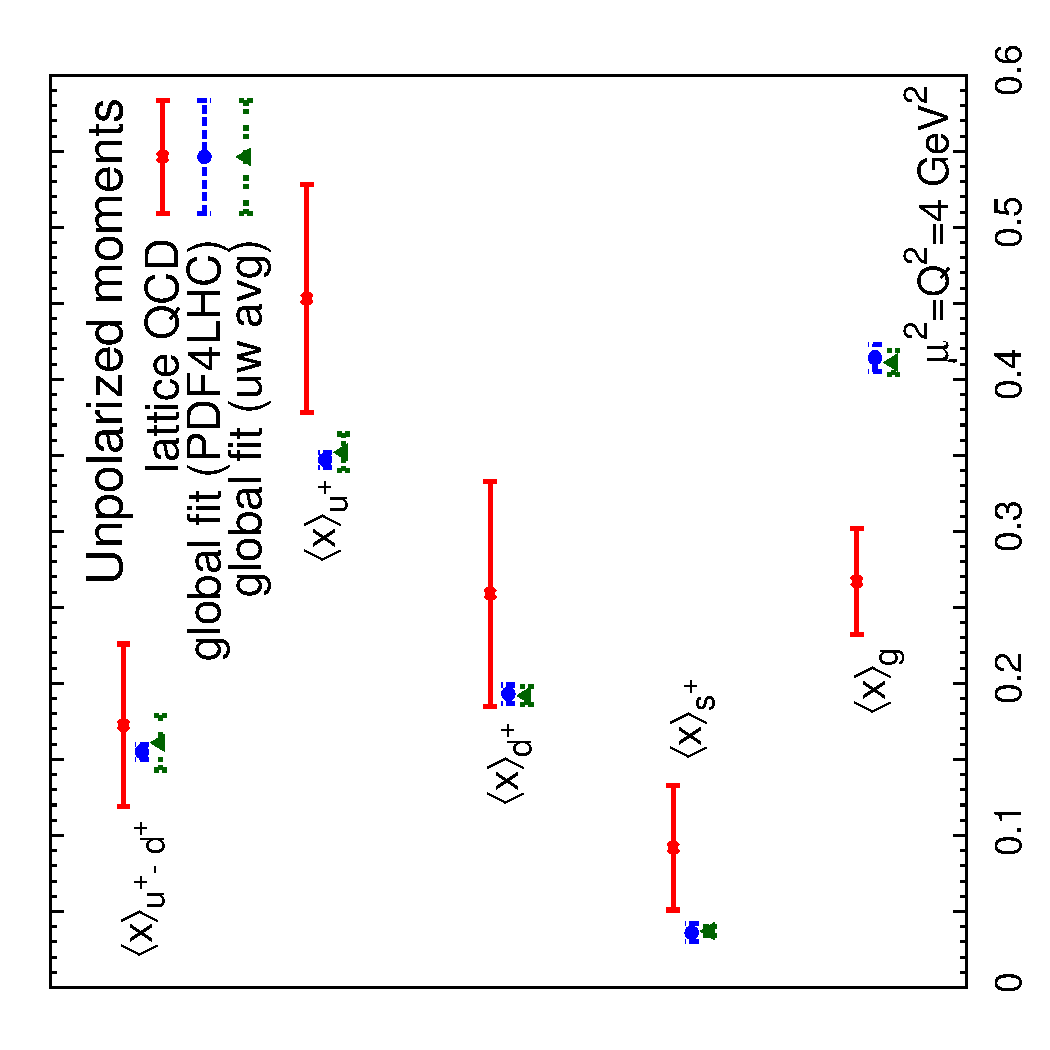
\includegraphics[scale=0.44,angle=270]{plots/unpmoms}
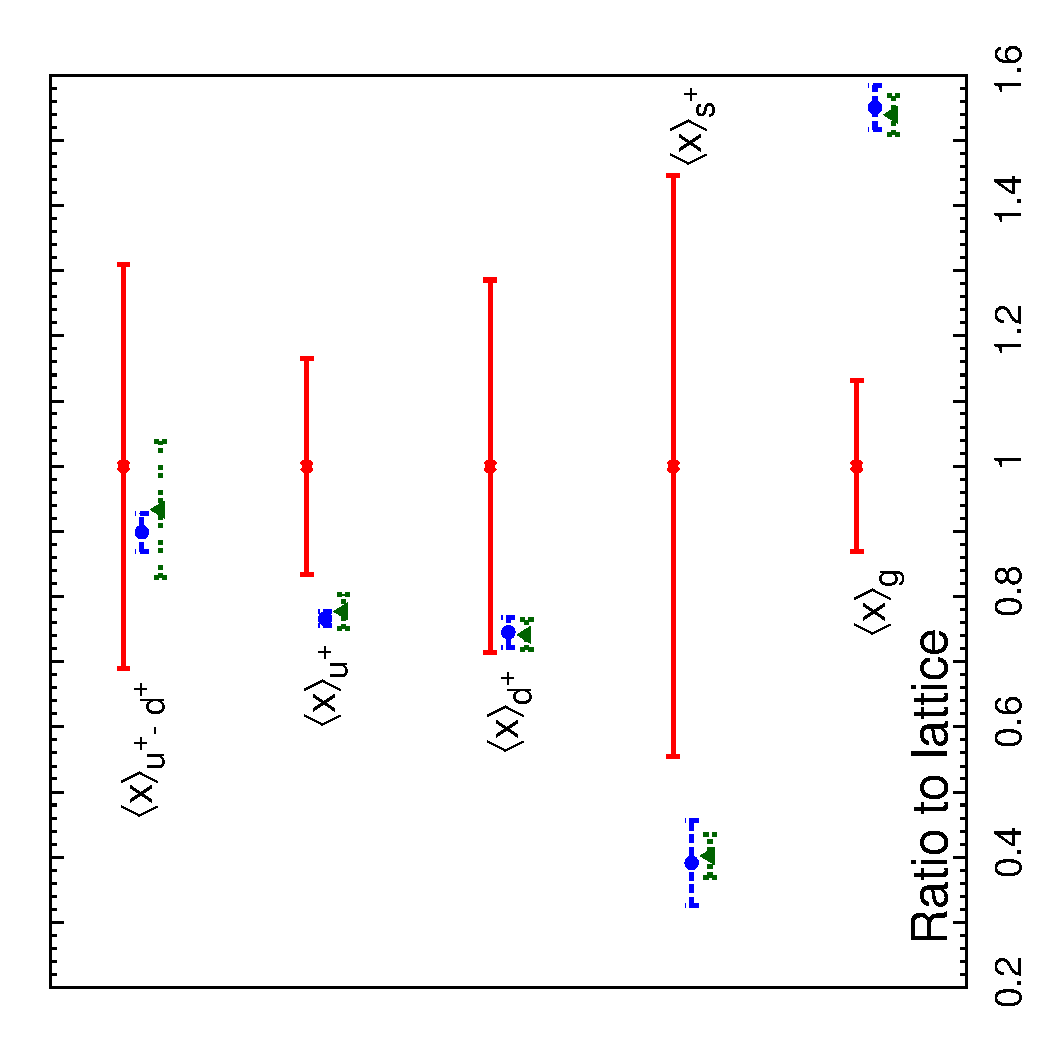
\includegraphics[scale=0.44,angle=270]{plots/unpmomsratio}\\
\caption{\small A comparison of the unpolarized PDF benchmark moments 
between the lattice QCD computations and global fit determinations.
%
Results are displayed both in terms of absolute values (left) and ratios to
the lattice values (right) at $\mu^2=4$ GeV$^2$.}
\label{fig:Bmomsunp}
\end{figure} 
%-------------------------------------------------------------------------------

As is apparent from Table~\ref{tab:BMunp} and Fig.~\ref{fig:Bmomsunp}, there is 
a significant difference in the uncertainties between the lattice QCD and 
global fit results, with the latter always about one order of magnitude 
smaller than the former.
%
Moreover, even within their large uncertainties, the lattice-QCD results 
for the first moments of the total up and strange quark and the gluon PDFs
are not compatible with their global-fit counterparts.
%
In the case of quarks, the discrepancy is below $2\sigma$ (in units of the 
lattice-QCD uncertainty), while in the case of the gluon the discrepancy is
slightly larger than $3\sigma$.

On the lattice-QCD side, we note that in the flavor-singlet sector calculations
neglected part of the renormalization and computed some other parts only 
perturbatively.
%
Most of the discrepancies between lattice-QCD and global-fit results are 
observed in the flavor-singlet sector.
%
Progress in taking into account the renormalization properly
could shift lattice-QCD results significantly, and reconcile them 
with the global fits in the future.
%
We also note that the momentum sum rule, Eq.~\eqref{eq:mom}, usually is not 
imposed in lattice-QCD calculations.
%
In the ETMC\,17 analysis~\cite{Alexandrou:2017oeh}, it turns
out to be $1.071(93)(72)$, see Table~\ref{tab:unpolLQCDstatus1}, if 
uncertainties are assumed to be uncorrelated.
%
Although there is no evidence for a violation of the momentum sum rule 
based on this result, one must be careful combining results from different 
calculations to account for correlations and other sources of error. 
%
Also, note that the ETMC\,17 analysis is performed with $N_f=2$ flavors,
hence the strange quark should not participate in the sum rule.

On the global-fit side, we note that the amount of experimental information 
that constrains the total up-quark distribution is the largest among all 
distributions.
%
Therefore, it seems unlikely that its global-fit central value could vary 
significantly in the future, and become compatible with the current
lattice result.
%
Conversely, the amount of experimental information that constrains the
total strange distribution in a global fit is less abundant and less accurate.
%
A slight shift in its central value, towards the current lattice-QCD results,
might be observed in the future, as soon as new data sensitive to the strange 
quark becomes available.
%
Finally, in an attempt to reconcile the lattice-QCD and the global-fit results
of the first moment of the gluon PDF, one could assume a completely
different behavior of the gluon PDF below the HERA kinematic
coverage, $x\sim 10^{-5}$ (see Fig.~\ref{fig:kinplot-report}).
%
While such a kinematic region remains completely unexplored,
in general the contribution of this region to the moments is negligible
and thus unlikely to resolve the situation. 

All these remarks apply irrespective of the benchmark value used for 
global fits, either the PDF4LHC or the unweighted average.
%
They also still hold if individual lattice-QCD and/or global-fit
results in Tables~\ref{tab:unpolLQCDstatus1}-\ref{tab:unpPDFmoms} are 
compared instead of their benchmark values in Table~\ref{tab:BMunp}. 
%
These results suggest that both greater accuracy and greater precision are
required in lattice-QCD calculations to match the accuracy and 
precision of the first moments of unpolarized PDFs determined from a global
fit.

\paragraph{Polarized parton distributions.}
%
The benchmark values of the first moments of the unpolarized PDFs, obtained
as described in Sects.~\ref{subsubsec:BClQCD}-\ref{subsubsec:GPDFfits}, 
are summarized in Table~\ref{tab:BMpol}.
%
Results from a single lattice calculation, which might underestimate some 
sources of uncertainty, are denoted with a superscript~$\dagger$.
%
In the case of $g_A$, we report the two values with $N_f=2+1+1$ and
$N_f=2$ sea quarks from lattice QCD.
%
The value of $g_A$ is scale-independent, and we quote all other results at 
$\mu^2=4\mbox{ GeV}^2$.
%
For ease of comparison, these values are also displayed in 
Fig.~\ref{fig:Bmomspol} in the same format as in Fig.~\ref{fig:Bmomsunp}.
%
In the case of $g_A$, the result with $N_f=2+1+1$ is used as normalization
factor in the right panel of Fig.~\ref{fig:Bmomspol}.
%
Results from the JAM17 analysis~\cite{Ethier:2017zbq}, see 
Table~\ref{tab:polPDFmoms}, are displayed separately.
%
In contrast with the NNPDFpol1.1, DSSV08 and JAM15 fits, in the JAM17 fit 
the experimental value of $g_A$, Eq.~\eqref{eq:a3}, 
is not an input of the PDF fit.

%-------------------------------------------------------------------------------
\begin{table}[!t]
\centering
\renewcommand{\arraystretch}{1.2}
\begin{tabular}{lcc}
\toprule
Moment & Lattice QCD & Global Fit\\
\midrule
\multirow{2}{*}{$g_A\equiv\langle 1\rangle_{\Delta u^+ - \Delta d^+}$} 
& 1.195(39) ($N_f=2+1+1$) 
& \multirow{2}{*}{\ 1.275(12)} \\
& 1.279(50) ($N_f=2$) & \\
$\langle 1 \rangle_{\Delta u^+}$     
& 0.830(26)$^\dagger$ 
& \ 0.813(25)\\
$\langle 1 \rangle_{\Delta d^+}$     
& -0.386(17)$^\dagger$ 
& -0.462(29)\\
$\langle 1 \rangle_{\Delta s^+}$     
& -0.052\,--\,-0.014
& -0.114(43)\\
$\langle x\rangle_{\Delta u^- - \Delta d^-}$       
& \numrange{0.146}{0.279} 
& \ 0.199(16)\\
\bottomrule
\end{tabular}
\caption{\small Same as Table~\ref{tab:BMunp}, but for the polarized benchmark 
moments.}
\label{tab:BMpol}
\end{table}
%-------------------------------------------------------------------------------

%-------------------------------------------------------------------------------
\begin{figure}[!t]
\centering
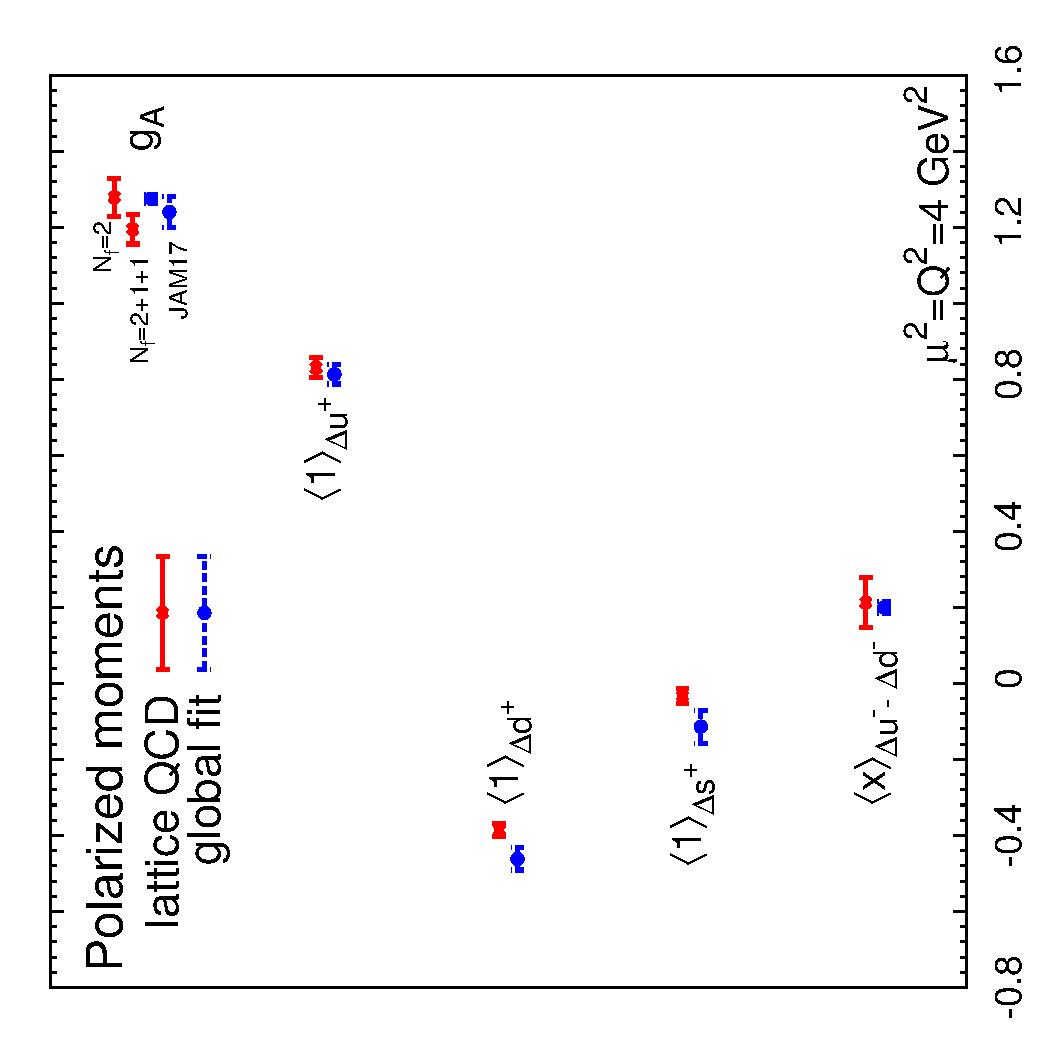
\includegraphics[scale=0.44,angle=270]{plots/polmoms}
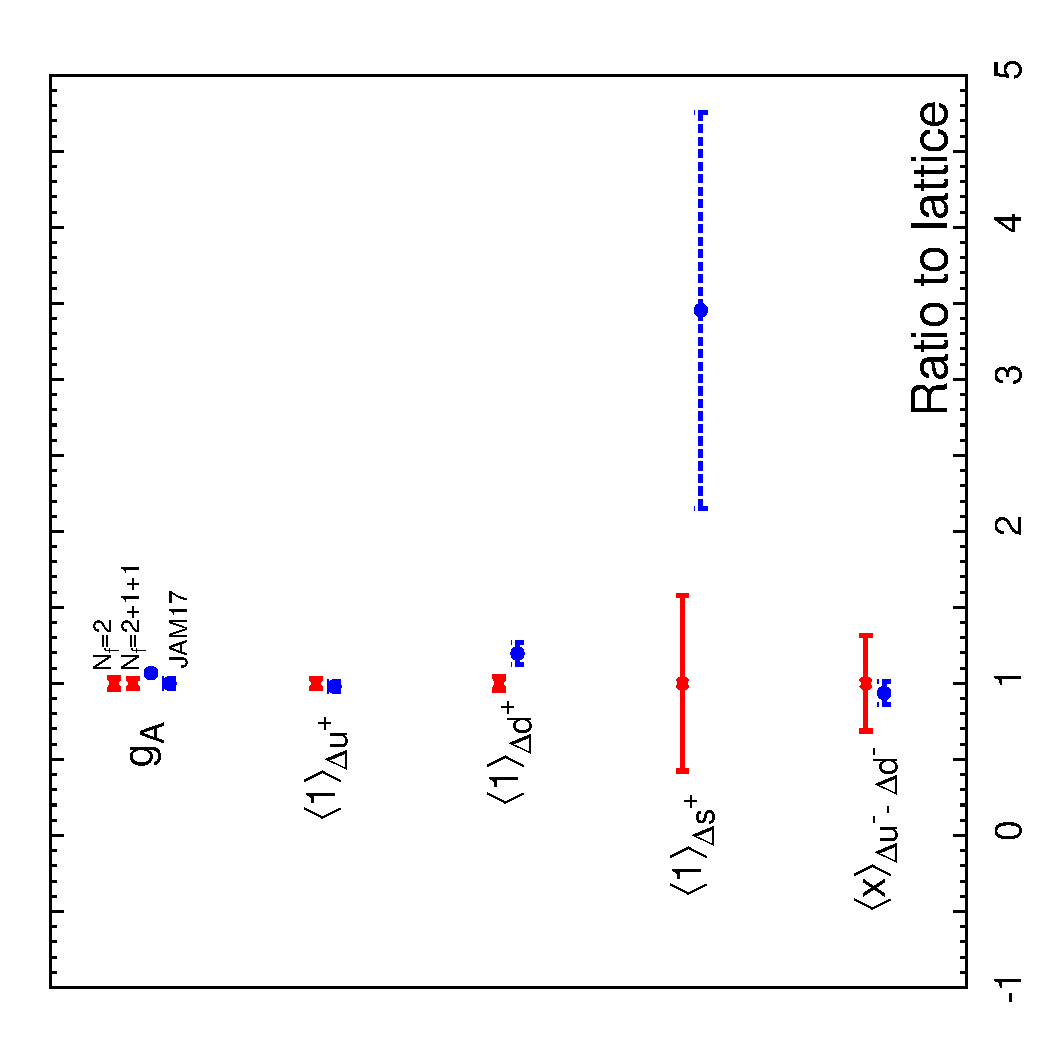
\includegraphics[scale=0.44,angle=270]{plots/polmomsratio}\\
\caption{\small Same as Fig.~\ref{fig:Bmomsunp}, but for the polarized
benchmark moments.}
\label{fig:Bmomspol}
\end{figure} 
%-------------------------------------------------------------------------------

As is apparent from Table~\ref{tab:BMpol} and Fig.~\ref{fig:Bmomspol}, the 
size of the uncertainties on the moments is in general comparable between the 
lattice-QCD and the global-fit results, opposite to the unpolarized case.
%
The corresponding central values are also in reasonable agreement within their
mutual uncertainties.

In the case of $g_A$, the global-fit result obtained from the unweighted 
average of the NNPDFpol1.1, DSSV08 and JAM15 fits shows a preference for the
lattice-QCD result obtained with $N_f=2$ sea quarks (compared to that with 
$N_f=2+1+1$ sea quarks).
%
Its uncertainty is, however, four times smaller than that of both lattice 
results.
%
This is not unexpected, since, in all the three fits that are combined, the 
experimental value of $g_A$ is imposed in the fits themselves.
%
The final uncertainty on the global-fit value of $g_A$ is thus reduced by 
the uncertainty of its experimental value $g_A^\text{exp}$, which is almost
one order of magnitude smaller than the uncertainty on the lattice-QCD results
(see Fig.~\ref{fig:gaLQCDstatus}).
%
If the experimental value of $g_A$ is not imposed as a boundary condition in 
the fit, as in the JAM17 analysis, the size of the uncertainty on $g_A$ is 
comparable to that of the lattice results, although it is not able to 
discriminate between the $N_f=2$ or the $N_f=2=1+1$ results.
%
Overall, this is a noteworthy confirmation of SU(2) symmetry in QCD to
almost 2\%.

In the case of the zeroth moments of the total polarized quark distributions,
the uncertainty on the lattice-QCD result is comparable to (in the case
of $\langle 1 \rangle_{\Delta u^+}$) or smaller than (in the case
of $\langle 1 \rangle_{\Delta d^+}$ and $\langle 1 \rangle_{\Delta s^+}$)
the uncertainty on the global-fit result.
%
However, in the case of the zeroth moments of the total down- and strange-quark 
distributions, the lattice-QCD and the global-fit results are discrepant
by about two $\sigma$ (in units of the
lattice QCD uncertainty).
%
On the one hand, we observe that the uncertainty on the lattice-QCD results 
might have been underestimated because of the lack of full control over
all systematics (see Sect.~\ref{subsubsec:BClQCD}).
%
On the other hand, we observe that the global-fit result has been obtained
by requiring SU(3) symmetry, {\it i.e.}, by imposing in the individual fits 
the experimental value (with a possibly inflated uncertainty) of the octet PDF 
combination, as explained in Sect.~\ref{sec:polPDFs}.
%
Relaxing this constraint can reconcile the discrepancy observed between 
the lattice-QCD and the global-fit result for the zeroth moments of the 
total down and strange PDFs.
%
This is demonstrated by comparison with the JAM17 result, whose uncertainty 
band nicely includes both the lattice-QCD and the global-fit benchmark values.

In the case of the first moment of the valence distribution 
$\Delta u^--\Delta d^-$, the lattice-QCD and the global-fit results are 
in excellent agreement, although the uncertainty of the former is five times
larger than that of the latter.

All these remarks still hold if individual lattice-QCD and/or global-fit
results in Tables~\ref{tab:gAstatus}-\ref{tab:polLQCDstatus0}-\ref{tab:polLQCDstatus1}-\ref{tab:polPDFmoms}
are compared instead of their benchmark values in Table~\ref{tab:BMpol}.
%
These results suggest that lattice-QCD calculations could provide a useful
input to global fits of polarized PDFs, especially in limiting the
extrapolation uncertainty into the completely unknown small-$x$ region.
%
This will become more and more useful as full control over all sources of
systematic uncertainties is achieved.
